\documentclass[lettersize,journal]{IEEEtran}
\usepackage{amsmath,amsfonts}
\usepackage[utf8]{inputenc} % allow utf-8 input
\usepackage[T1]{fontenc}    % use 8-bit T1 fonts
\usepackage{hyperref}       % hyperlinks
\usepackage{url}            % simple URL typesetting
\usepackage{booktabs}       % professional-quality tables
\usepackage{amsfonts, amsmath}       % blackboard math symbols
\usepackage{nicefrac}       % compact symbols for 1/2, etc.
\usepackage{microtype}      % microtypography
\usepackage{xcolor}         % colors
\usepackage{graphicx}
\usepackage{algorithmic}
\usepackage{algorithm}
\usepackage{array}
% \usepackage[caption=false,font=normalsize,labelfont=sf,textfont=sf]{subfig}
\usepackage{subcaption}
\usepackage{textcomp}
\usepackage{stfloats}
\usepackage{url}
\usepackage{verbatim}
\usepackage{graphicx}
\usepackage{bm}
\usepackage{newfloat}
\usepackage{listings}
\usepackage{makecell}
\usepackage{enumitem,kantlipsum}
\usepackage{empheq}
\usepackage{wrapfig}
\usepackage[numbers]{natbib}
\usepackage{scalerel}
\usepackage{multirow}
\usepackage{booktabs}
\usepackage{lipsum}
\usepackage{titlesec}
\usepackage{tabularx}

% \titlespacing\section{0pt}{12pt plus 4pt minus 2pt}{0pt plus 2pt minus 2pt}
\titlespacing\subsection{0pt}{12pt plus 0pt minus 2pt}{0pt plus 2pt minus 2pt}
% \titlespacing\subsubsection{0pt}{12pt plus 4pt minus 2pt}{0pt plus 2pt minus 2pt}

\hyphenation{op-tical net-works semi-conduc-tor IEEE-Xplore}
% updated with editorial comments 8/9/2021

\begin{document}

\title{
  % AgentMatrix: Building Distributed and Scalable LM Systems with Nested Agent
  % AgentMatrix: Building Nested and Distributed Mulit-Agent LLM Systems with Scalability and Flexibility
  % AgentMatrix: A Nested and Distributed Mulit-Agent LLM Systems with Scalability and Flexibility
  % AgentMatrix: A New-Generation Nested and Distributed Mulit-Agent LLM Systems
  % AgentMatrix: Advancing Scalable and Distributed Multi-Agent LLM Infrastructures with Nested Architecture
  AgentMatrix: Advancing towards Nested and Distributed Multi-Agent LLM Infrastructures
}
\author {
    Qingxu Fu
    \thanks{
    The authors are with the Institute of Automation, Chinese Academy of Sciences, Beijing 100190, China,
    the School of Artificial Intelligence, University of Chinese Academy of Sciences, Beijing 100049, China.
    (e-mail: fuqingxu2019@ia.ac.cn).
    }% <-this % stops a space
}


\maketitle

\begin{abstract}
  Recent advances in Large Language Models (LLMs) have propelled substantial developments in artificial intelligence (AI).
Many researchers have leveraged LLMs as the foundation to build AI agent systems for two primary purposes: a) developing robust, efficient and user-friendly applications to overcome LLMs' performance and input-domain limitations. b) refining datasets or reward models from existing datasets and LLMs, thereby augmenting the capability of LLMs in a ``bootstrapping'' way.
Nevertheless, the existing LLM-agent frameworks have many limitations,
such as the dependence on specific LLMs from certain companies, the lack of adaptability for novel scenarios, the insufficient scalability for extensive agent interactions, and the inability to respond in real time to user inputs like audio.
To address these problems, we propose AgentMatrix, a multi-agent framework for LLM-based agents. AgentMatrix features a nested and distributed design: (1) The agents can be joined together by Directed Acyclic Graphs (DAGs), Directed Cyclic Graphs (DCGs), or autonomous free chat groups, thus composing into higher-level agents with stronger capability. Furthermore, the composed agents can join with agents (of any level) once again, forming a sophisticated and well-organized nested structure. (2) Different agents can be distributed into different physical devices, allowing the user terminal devices to integrate agents with high resource consumptions and prompting the scalability and flexibility of the system. AgentMatrix is accessible at \url{https://github.com/binary-husky/agent-matrix/}.
\cite{wolpert1997no}\cite{wolpert1997no}

% E.g., high dependency on specific LLMs from specific companies, lacking the flexibility to address problems in new scenarios, lacking the scalability to allow large-scale agent interaction, and lacking the capability to make real-time responses toward user inputs such as audio.


% Recent advances in Large Language Models (LLMs) have catalyzed substantial progress in artificial intelligence (AI). Numerous researchers utilize LLMs as a foundation to engineer AI agents for two principal objectives: a) enhancing application robustness, efficiency, and user-friendliness to surmount limitations in LLM performance and input domains; b) refining datasets and reward models derived from extant datasets and LLMs, thereby augmenting LLM capabilities through iterative enhancement. However, the extant AI agent frameworks exhibit significant limitations, such as dependence on specific LLMs from certain companies, a lack of adaptability for novel scenarios, insufficient scalability for extensive agent interactions, and an inability to respond in real time to user inputs like audio. To surmount these challenges, we introduce AgentMatrix, a versatile multi-agent framework designed for LLM-based agents. AgentMatrix boasts a nested and distributed architecture, enabling: a) agent integration into higher-level constructs via Directed Acyclic Graphs, Directed Cyclic Graphs, or autonomous chat groups, which further amalgamate to form sophisticated, nested structures; b) agent distribution across various physical devices, enhancing system scalability and flexibility while enabling resource-heavy agents to integrate with user terminals. AgentMatrix is available at


% Recent advances in Large Language Models (LLMs) have propelled substantial developments in artificial intelligence (AI). Researchers widely adopt LLMs to craft AI agents with two principal objectives: firstly, to enhance robustness, efficiency, and user accessibility in applications that transcend the inherent performance and domain constraints of LLLMs; and secondly, to curate superior datasets or refinement models which in turn augment the competencies of LLMs through iterative self-improvement. Despite these strides, contemporary AI agent paradigms exhibit several shortcomings, including over-reliance on select LLMs exclusive to certain corporations, restricted adaptability for emergent scenarios, limited interaction scalability, and inadequate instantaneous responsiveness to user inputs, such as audio signals. To mitigate these challenges, we introduce AgentMatrix, a multi-agent framework engineered for LLM-centric AI agents. AgentMatrix distinguishes itself with a nested, distributed architecture: agents can be interconnected through various configurations, such as Directed Acyclic Graphs (DAGs), Directed Cyclic Graphs (DCGs), or self-governing chat ensembles, enabling the formation of advanced, multi-tier agents. This modular structuring further permits intricate nesting of composed agents, yielding an organized, versatile system. Moreover, the framework's distributed nature allows for agents to be deployed across diverse hardware, enhancing scalability and resource allocation for end-user devices. AgentMatrix is accessible at \url{https://github.com/binary-husky/agent-matrix/}.


% and have achieved significant progress,
% nevertheless, the potential of LLMs is far from being fully explored.

% However, the complexities in coordinating agents’ cooperation and LLMs’ erratic performance pose notable challenges in developing robust and efficient multi-agent applications.

% Agents are the basic unit to process the information flow in AgentMatrix.

% , comprising three main components:
% brain, perception, and action, and the framework can be tailored for different
% applications. Subsequently, we explore the extensive applications of LLM-based
% agents in three aspects: single-agent scenarios, multi-agent scenarios, and humanagent cooperation.


% With the rapid advancement of Large Language Models (LLMs), significant progress has been made
% in multi-agent applications. However, the complexities in coordinating agents’ cooperation and LLMs’
% erratic performance pose notable challenges in developing robust and efficient multi-agent applications.
% To tackle these challenges, we propose AgentScope, a developer-centric multi-agent platform with
% message exchange as its core communication mechanism. Together with abundant syntactic tools, builtin resources, and user-friendly interactions, our communication mechanism significantly reduces the
% barriers to both development and understanding. Towards robust and flexible multi-agent application,
% AgentScope provides both built-in and customizable fault tolerance mechanisms while it is also armed
% with system-level supports for multi-modal data generation, storage and transmission. Additionally, we
% design an actor-based distribution framework, enabling easy conversion between local and distributed
% deployments and automatic parallel optimization without extra effort. With these features, AgentScope
% empowers developers to build applications that fully realize the potential of intelligent agents. We have
% released AgentScope at https://github.com/modelscope/agentscope, and hope AgentScope invites
% wider participation and innovation in this fast-moving field.


\end{abstract}

\begin{IEEEkeywords}
Multi-agent systems, nested agents, large language models, supervised fine-tuning, reinforcement learning.
\end{IEEEkeywords}


\begin{figure*}[ht]
  \centering
  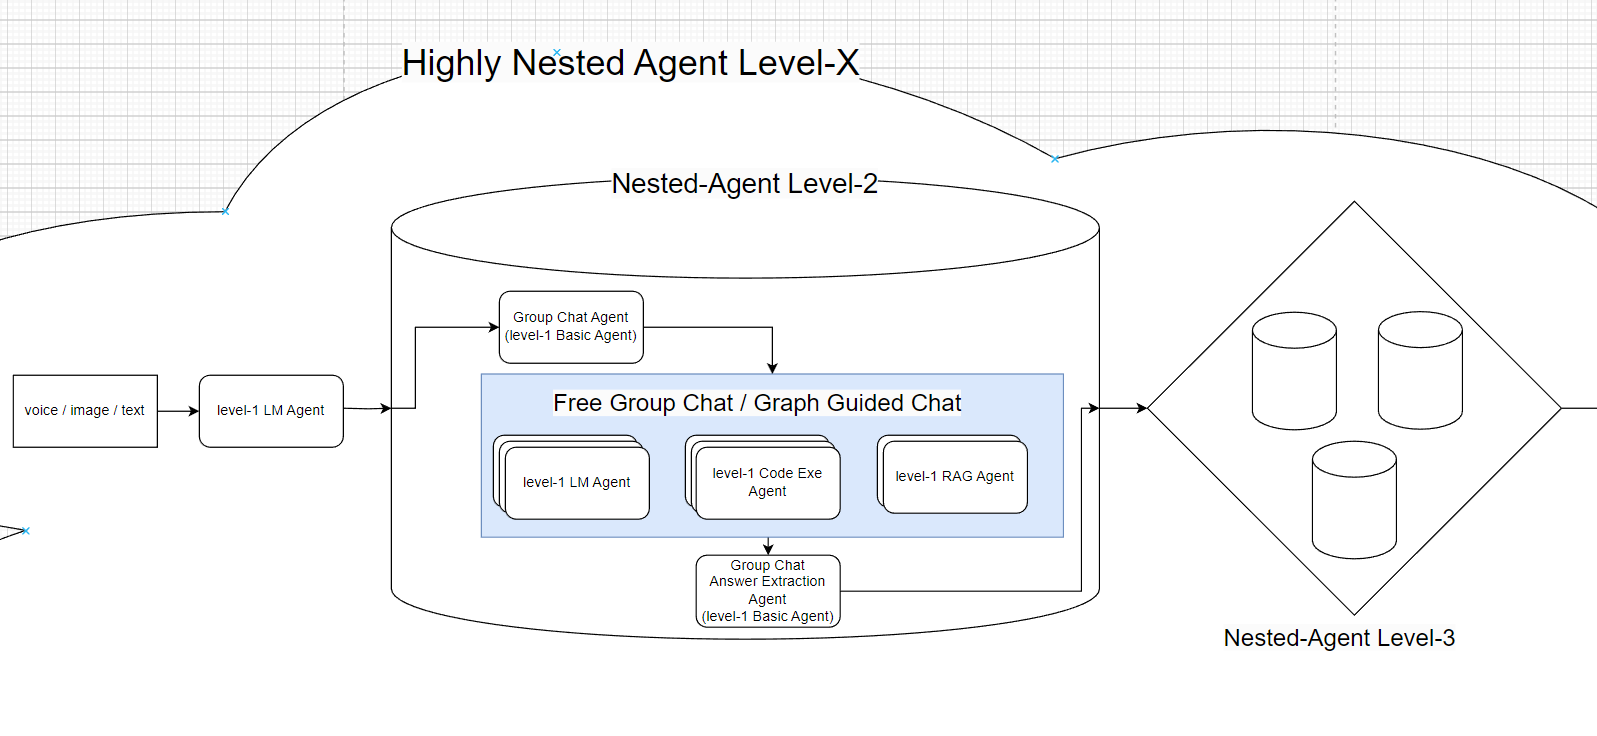
\includegraphics[width=0.9\linewidth]{drawio/299397865-1e63278f-0453-4b84-83c7-deb7c92ac466.png}
  \caption{Agents are allowed to establish nested cooperation structure in AgentMatrix.}
  \label{fig:agent_nestded}
  \end{figure*}

\begin{figure*}[ht]
  \centering
  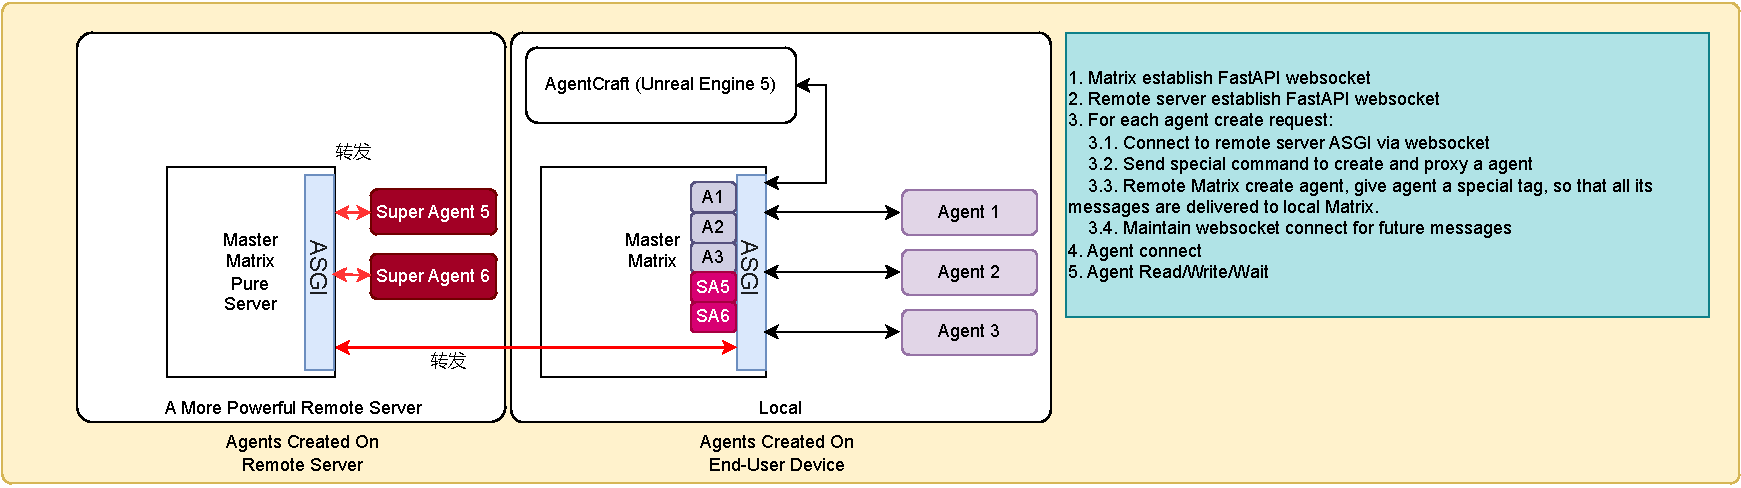
\includegraphics[width=0.9\linewidth]{drawio/distributed-phase2.drawio.pdf}
  \caption{The communication and distribution of agents in AgentMatrix framework.}
  \label{fig:agent_com}
  \end{figure*}

\begin{figure*}[ht]
  \centering
  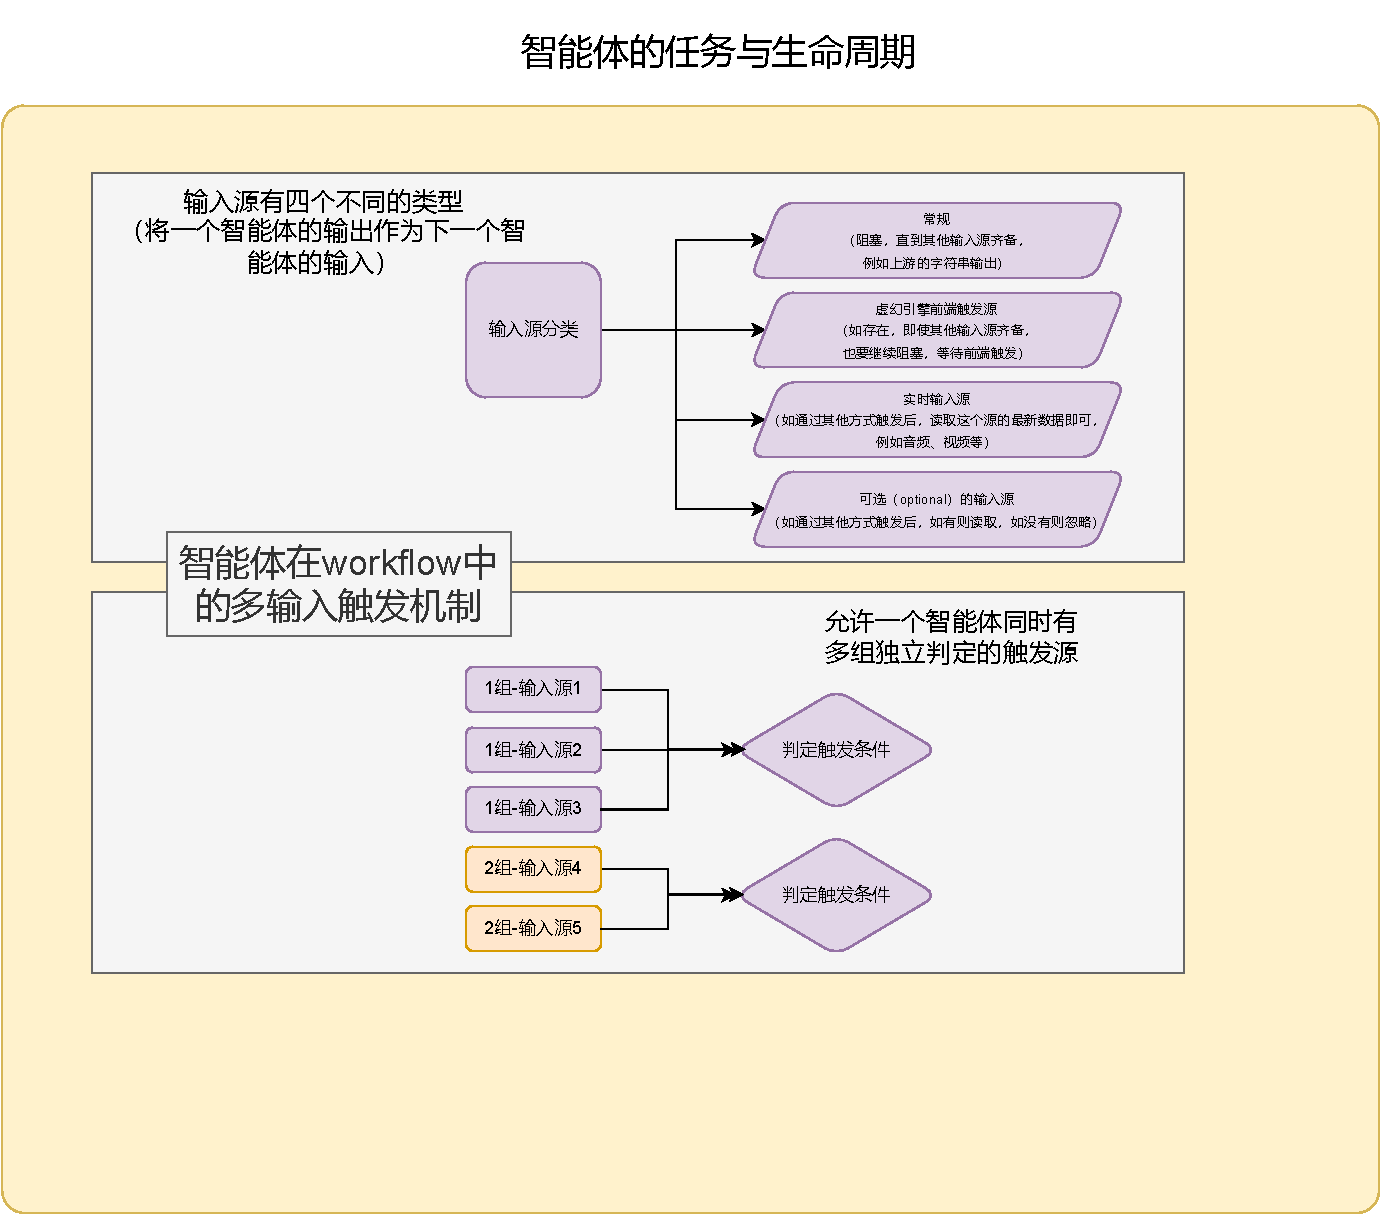
\includegraphics[width=0.9\linewidth]{drawio/agent_trigger.drawio.pdf}
  \caption{Agent begin its task when receiving triggers. In most cases, agents should begin working when it receives message from its upsteam agents. However, an agent can connect to multiple upsteam agents simutanously, and in some applications an agent also has to deal with real-time signal. Thereby, a multi-group triggering mechanism is designed to resolve these challenges.}
  \label{fig:agent_trigger}
  \end{figure*}



\bibliographystyle{IEEEtranN}

{\footnotesize
\bibliography{cite.bib}}




\vfill

\end{document}


